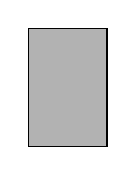
\begin{tikzpicture}
    %\pgfmathsetmacro{\cubex}{1}
    %\pgfmathsetmacro{\cubey}{2}
    %\pgfmathsetmacro{\cubez}{2}
    %\draw (0,0,0) -- (\cubex,0,0);
    %\draw (0,0,0) -- (0,\cubey,0);
    %\draw (0,\cubey,0) -- (\cubex,\cubey,0);
    %\draw (\cubex,0,0) -- (\cubex,\cubey,0);
    %\draw [dashed] (0,0,-\cubez) -- (\cubex,0,-\cubez);
    %\draw [dashed] (0,0,-\cubez) -- (0,\cubey,-\cubez);
    %\draw (0,\cubey,-\cubez) -- (\cubex,\cubey,-\cubez);
    %\draw (\cubex,0,-\cubez) -- (\cubex,\cubey,-\cubez);
    %\draw [dashed] (0,0,0) -- (0,0,-\cubez);
    %\draw (0,\cubey,0) -- (0,\cubey,-\cubez);
    %\draw (\cubex,\cubey,0) -- (\cubex,\cubey,-\cubez);
    %\draw (\cubex,0,0) -- (\cubex,0,-\cubez);
    \pgfmathsetmacro{\cubex}{1}
    \pgfmathsetmacro{\cubey}{1.5}
    \pgfmathsetmacro{\cubez}{1.5}
    \draw[fill=gray!60!] (2.5,0.75,0) -- ++(-\cubex,0,0) -- ++(0,-\cubey,0) -- ++(\cubex,0,0) -- cycle;
    %\draw[fill=gray!80!] (2.5,0.75,0) -- ++(0,0,-\cubez) -- ++(0,-\cubey,0) -- ++(0,0,\cubez) -- cycle;
    %\draw[fill=gray!50!] (2.5,0.75,0) -- ++(-\cubex,0,0) -- ++(0,0,-\cubez) -- ++(\cubex,0,0) -- cycle;
    %\draw[blue!60!cyan!90!, -{Triangle[width = 14pt, length = 8pt]}, line width = 6pt] (2.7, 0.) -- (3.7, 0);
    %\draw[blue, -{Triangle[width = 14pt, length = 8pt]}, line width = 6pt] (0.0, 0.0) -- (1, 0.0);
    %\node at (-0.3,0) {$I_{\nu}$};
    %\node at (4.5,0) {$I_{\nu} + dI_{\nu}$};
    %\draw (1,-0.8) -- (1,-0.9) -- (2.5,-0.9) -- (2.5,-0.8);
    %\node at (1.75,-1.1) {$dx$};
    %\node at (2,0) {$\kappa_{\nu}$};
\end{tikzpicture}